% Supplementary material of the FastPose-ViT-MO paper: a SEPARATE document from main.tex (CVF
% conferences take the supplementary as its own PDF). Same preamble, notation and bibliography.
% Compile this file on its own (Overleaf: Menu -> Main document -> supplementary.tex, or a second
% project). Sections are numbered S1, S2, ...; the main paper refers to them as "Supp. Sec. Sx".
% Figures come from paper/figures (scripts vis/paper_*.py); numbers from docs/BOP.md and
% TASKS.md §9. Status (2026-11-14): bbox jitter 5 / 15 / 30 % (seed a) and T-LESS still running.
% Shared preamble of main.tex and supplementary.tex (same packages, macros and notation).
\documentclass[10pt,twocolumn,letterpaper]{article}

\IfFileExists{wacv.sty}{%
  \usepackage[review]{wacv}
  \def\paperID{*****}
  \def\confName{WACV}
  \def\confYear{2027}
}{%
  \usepackage[margin=0.75in,columnsep=0.25in]{geometry}
  \usepackage{times}
}

\usepackage{amsmath,amssymb,bm}
\usepackage{graphicx}
\usepackage{booktabs}
\usepackage{multirow}
\usepackage{xcolor}
\usepackage[hidelinks]{hyperref}
\usepackage[capitalize]{cleveref}

% Draft helpers: \pending for results still running, \todo for things to write or check.
\newcommand{\pending}[1]{\textcolor{orange}{[\textbf{Pending:} #1]}}
\newcommand{\todo}[1]{\textcolor{red}{[\textbf{TODO:} #1]}}
\newcommand{\figplaceholder}[2]{\fbox{\parbox[c][#1][c]{0.95\linewidth}{\centering\small #2}}}

% Notation (\eg is defined by the WACV style; fallback otherwise)
\providecommand{\eg}{e.g.\@\xspace}
\usepackage{xspace}
\newcommand{\R}{\mathbf{R}}
\newcommand{\T}{\mathbf{T}}
\newcommand{\K}{\mathbf{K}}
\newcommand{\U}{\mathbf{U}}
\newcommand{\ours}{FastPose-ViT-MO}


\renewcommand{\thesection}{S\arabic{section}}
\renewcommand{\thetable}{S\arabic{table}}
\renewcommand{\thefigure}{S\arabic{figure}}
\renewcommand{\theequation}{S\arabic{equation}}

\title{\ours: Real-Time Multi-Object 6D Pose Estimation by Direct Regression\\
\large Supplementary Material}
\author{Pablo Sarro\\ EPFL}

\begin{document}
\maketitle

This document complements the main paper with implementation details (\cref{sec:supp:impl}),
the handling of symmetric objects (\cref{sec:supp:sym}), the complete ablation tables
(\cref{sec:supp:ablations}), the detection quality (\cref{sec:supp:det}), deployment details
(\cref{sec:supp:deploy}), an analysis of the depth bias on YCB-V (\cref{sec:supp:depth}),
per-object results (\cref{sec:supp:perobject}), reproducibility information
(\cref{sec:supp:repro}), and an RGB-D variant (\cref{sec:supp:rgbd}). Unless stated otherwise, AR is the official BOP19 average recall on the
LM-O test set with the default detections of the BOP 2023 challenge, and ``seed a / b'' are two
training runs that differ only in the random seed of the object-balanced sampler.

% ---------------------------------------------------------------------------------------------
\section{Implementation details}
\label{sec:supp:impl}

\paragraph{Hyperparameters.}
\Cref{tab:supp:hparams} lists the configuration of the final models. Ablations use the same
configuration with half the samples per epoch (2$\times$).

\begin{table}[h]
  \centering
  \footnotesize
  \begin{tabular}{ll}
    \toprule
    Setting & Value \\
    \midrule
    Backbone & ViT-B/16, $384 \times 384$ input, SWAG weights~\cite{singh2022swag} \\
    Head & one linear layer on the class token, 9 outputs ($\U$, 6D $\R'$) \\
    Object conditioning & class token $\mathbf{c} + \mathbf{e}_k$, $\mathbf{e}_k$ initialized at 0 \\
    Optimizer & Muon~\cite{jordan2024muon} for matrix parameters (incl.\ $\mathbf{e}_k$), \\
     & AdamW ($\beta = 0.9, 0.95$, $0.1\times$ LR) for 1-D parameters; no weight decay \\
    Learning rate & $8 \cdot 10^{-4} \rightarrow 8 \cdot 10^{-6}$ ($10^{-4}$ at batch 4, scaled linearly) \\
    Schedule & cosine warm restarts, $T_0 = 10$ epochs, $T_\mathrm{mult} = 2$, per iteration \\
    Epochs, batch size & 150, 32 \\
    Samples per epoch & 21,104 per object (4$\times$); 10,552 (2$\times$) \\
    Precision & mixed (FP16 autocast, gradient scaling), \texttt{torch.compile} \\
    Losses & relative L2 on $\U$ + symmetric relative Frobenius on 6D $\R'$, weights 1 : 1 \\
    Crops & square of side $\max(w, h)$ around \texttt{bbox\_visib}, one affine warp \\
    Box perturbation & $p = 0.5$, each side by up to 10\,\% of the box size \\
    Pixel augmentation & ``domain gap'' set, each operation with $p = 0.5$ \\
    Training instances & visible fraction $\geq 0.1$, PBR scenes 0--47 \\
    Validation & up to 2,000 instances of PBR scenes 48--49 (LM-O: and real \\
     & LM images of the 8 objects), score $(\mathrm{AR}_\mathrm{MSSD} + \mathrm{AR}_\mathrm{MSPD})/2$ \\
    Reported weights & last epoch (same AR as the best validation epoch) \\
    Hardware & 1 NVIDIA A100 80\,GB, 16 CPU cores per run \\
    Training time & LM-O 4$\times$ $\approx$ 34\,h; YCB-V 4$\times$ $\approx$ 58\,h; 2$\times$ ablation $\approx$ 12--17\,h \\
    \bottomrule
  \end{tabular}
  \caption{\textbf{Training configuration} of the final models.}
  \label{tab:supp:hparams}
\end{table}

\paragraph{Data.}
LM-O: 320,959 training instances of the 8 test objects in the LM PBR scenes 0--47; YCB-V: 626,520
instances of 21 objects; T-LESS: 666,063 instances of 30 objects. On T-LESS, an image can contain
more instances of an object than the BOP19 test targets list; we evaluate the most visible ones, as
many as the target count.

\paragraph{Pixel and box conventions.}
BOP boxes $[x, y, w, h]$ span the pixels $x$ to $x + w$ inclusive, and pixel $i$ is centred at
$i + 0.5$ in the coordinates of $\K$. We convert every ground-truth and detected box to
$[x, y, x + w + 1, y + h + 1]$ and map it to the crop with one affine warp that accounts for the
half-pixel offsets, so that the box centre lands exactly on the crop centre and the projected
object centre lands where $\U$ says (checked to $10^{-5}$ pixels). Areas of the square crop
outside the image are filled with zeros.

\paragraph{Pixel augmentations.}
The ``domain gap'' set applies each of the following Albumentations operations independently with
probability $p = 0.5$: grayscale, random tone curve, gamma, CLAHE, brightness and contrast,
solarize, sun flare, ISO noise, motion blur, defocus, and one of JPEG compression or downscaling.
The subsets of the augmentation study (\cref{tab:supp:aug}) are: \emph{color} = brightness and
contrast, gamma, hue and saturation; \emph{blur} = Gaussian ($3$--$7$\,px), motion and defocus
blur; \emph{noise} = Gaussian (standard deviation 0.02--0.1) and ISO noise; each operation with
$p = 0.5$.

\paragraph{No in-plane rotation augmentation.}
FastPose-ViT rotates the image about its centre and relabels the pose with the corresponding
camera roll. This is exact only if the rotation centre is the principal point and $f_x = f_y$.
On LM, the principal point is about $(5.8, 2.6)$\,px from the image centre and $f_x \neq f_y$,
which gives label errors of about 20\,mm at a rotation of 180\textdegree. An exact variant would
warp the image with $\K \mathbf{R}_z(\theta) \K^{-1}$ and relabel $\T' = \mathbf{R}_z \T$,
$\R' = \mathbf{R}_z \R$; we do not use it.

\paragraph{Detector.}
The multi-class LW-DETR~\cite{chen2024lwdetr} uses the original recipe: group DETR with 13 query
groups in training (one at inference), IoU-aware classification loss, loss weights 1 / 5 / 2
(classification / L1 / GIoU), AdamW with learning rate $10^{-4}$ ($1.5 \cdot 10^{-4}$ for the
encoder), weight decay $10^{-4}$, 500 warm-up iterations, EMA decay 0.9997, gradient clipping at
0.1, COCO-pretrained weights except the class head, BF16 training. Images are resized to
$640 \times 640$; augmentations are the ``domain gap'' set and horizontal flips. We train for 50
epochs on the 48,000 LM PBR images (batch 32) and keep the checkpoint with the best COCO mAP on
the held-out PBR scenes; training takes about 12\,h (tiny) and 22\,h (small) on one A100.

% ---------------------------------------------------------------------------------------------
\section{Symmetric objects}
\label{sec:supp:sym}
The symmetry transformations come from the BOP model information (\texttt{models\_info.json}) via
the BOP toolkit; continuous symmetries are discretized with a step of 1\,\% of the object diameter,
and the symmetry table of each dataset is padded with the identity (a repeated identity does not
change the minimum of the loss). On LM-O, the eggbox and the glue have one flip each; the flips of
the scanned models are not exactly 180\textdegree\ (179.8\textdegree\ and 178.5\textdegree), and we
use them as given, as the BOP19 evaluation does. On YCB-V, two objects have continuous symmetries,
and the symmetry of the two clamps shifts the model by about 19\,mm: without the translation
offsets of Sec.~3.4 of the main paper, a 256-instance overfitting check reaches
only 0.91 and 0.88 (score $(\mathrm{AR}_\mathrm{MSSD} + \mathrm{AR}_\mathrm{MSPD})/2$) on the
clamps, and 1.000 for all 21 objects with them. On T-LESS, 27 of the 30 objects are symmetric (11
with continuous symmetries), with up to 315 discrete symmetries and offsets up to 14\,mm; the same
check reaches 1.000 on all 30 objects.

% ---------------------------------------------------------------------------------------------
\section{Complete ablation results}
\label{sec:supp:ablations}
All rows: one change from the ablation baseline (class token, 2$\times$, symmetric loss,
``domain gap'', 10\,\% box perturbation, size-invariant depth, SWAG, apparent rotation); AR per
seed, then the mean of the AR and of its three components over the two seeds.

\begin{table}[h]
  \centering
  \setlength{\tabcolsep}{3.5pt}
  \footnotesize
  \begin{tabular}{lccccc}
    \toprule
    Change & AR (a / b) & AR & VSD & MSSD & MSPD \\
    \midrule
    \textbf{none (baseline)} & 0.655 / 0.655 & 0.655 & 0.475 & 0.621 & 0.869 \\
    absolute rotation & 0.546 / 0.548 & 0.547 & 0.379 & 0.505 & 0.757 \\
    random initialization & 0.516 / 0.517 & 0.517 & 0.330 & 0.449 & 0.771 \\
    legacy depth & 0.610 / 0.625 & 0.617 & 0.409 & 0.598 & 0.845 \\
    \bottomrule
  \end{tabular}
  \caption{\textbf{Targets and pre-training} with the AR components. The absolute rotation and
  the random initialization hurt all three metrics; the legacy depth mostly hurts VSD.}
  \label{tab:supp:targets}
\end{table}

\begin{table}[h]
  \centering
  \setlength{\tabcolsep}{3.5pt}
  \footnotesize
  \begin{tabular}{lccccc}
    \toprule
    Box perturbation & AR (a / b) & AR & VSD & MSSD & MSPD \\
    \midrule
    0\,\% & 0.625 / 0.625 & 0.625 & 0.439 & 0.577 & 0.858 \\
    5\,\% & \pending{} & & & & \\
    \textbf{10\,\%} & \textbf{0.655 / 0.655} & \textbf{0.655} & 0.475 & 0.621 & 0.869 \\
    15\,\% & \pending{} / 0.651 & & & & \\
    20\,\% & 0.650 / 0.651 & 0.650 & 0.467 & 0.613 & 0.871 \\
    30\,\% & \pending{} / 0.643 & & & & \\
    \bottomrule
  \end{tabular}
  \caption{\textbf{Bounding-box perturbation} during training (each side by up to the given
  fraction of the box size, $p = 0.5$). Seed b of 15\,\% and 30\,\%: VSD / MSSD / MSPD 0.470 /
  0.615 / 0.869 and 0.458 / 0.602 / 0.868.}
  \label{tab:supp:bbox}
\end{table}

\begin{table}[h]
  \centering
  \setlength{\tabcolsep}{3.5pt}
  \footnotesize
  \begin{tabular}{lccccc}
    \toprule
    Pixel augmentation & AR (a / b) & AR & VSD & MSSD & MSPD \\
    \midrule
    none & 0.626 / 0.629 & 0.627 & 0.444 & 0.573 & 0.866 \\
    color & 0.649 / 0.641 & 0.645 & 0.463 & 0.602 & 0.870 \\
    blur & 0.628 / 0.630 & 0.629 & 0.445 & 0.577 & 0.865 \\
    noise & 0.627 / 0.627 & 0.627 & 0.444 & 0.574 & 0.864 \\
    color + blur + noise & 0.641 / 0.643 & 0.642 & 0.461 & 0.599 & 0.866 \\
    \textbf{domain gap, $p = 0.5$} & \textbf{0.655 / 0.655} & \textbf{0.655} & 0.475 & 0.621 & 0.869 \\
    domain gap, $p = 0.8$ & 0.641 / 0.631 & 0.636 & 0.456 & 0.594 & 0.859 \\
    \bottomrule
  \end{tabular}
  \caption{\textbf{Pixel augmentation study}. Augmentation acts mostly on the 3D metrics (VSD,
  MSSD); the 2D metric MSPD varies by at most 0.011. Without augmentation, the glue loses the most
  (0.67 $\rightarrow$ 0.53 AR) and the can follows (0.80 $\rightarrow$ 0.75).}
  \label{tab:supp:aug}
\end{table}

\begin{table}[h]
  \centering
  \setlength{\tabcolsep}{3.5pt}
  \footnotesize
  \begin{tabular}{llc}
    \toprule
    Study & Setting & AR (a / b) \\
    \midrule
    Training budget & 1$\times$ / 2$\times$ / 4$\times$ (heads) & 0.641 / 0.637, 0.650 / 0.650, 0.661 \\
    & 2$\times$ / \textbf{4$\times$} (token, YCB-V) & 0.681 / 0.689, \textbf{0.694 / 0.702} \\
    Augmentation set (heads, 1$\times$) & standard / \textbf{domain gap} & 0.629 / 0.645, \textbf{0.641 / 0.637} \\
    Symmetric rotation loss & off / \textbf{on} & 0.659 / 0.651, \textbf{0.655 / 0.655} \\
    Training crop & \textbf{visible} / amodal / mix & \textbf{0.655 / 0.655}, 0.646 / 0.650, 0.650 / 0.654 \\
    Conditioning & heads / \textbf{token} / both & 0.650 / 0.650, \textbf{0.659 / 0.651}, 0.660 / 0.661 \\
    Models & \textbf{one shared (4$\times$)} / 8 single-object & \textbf{0.669 / 0.664}, 0.672 \\
    Checkpoint & best validation / \textbf{last epoch} & 0.6686 / \textbf{0.6685} (YCB-V 0.7021 both) \\
    Precision & PyTorch / \textbf{TensorRT FP16} & 0.6685 / \textbf{0.6685} (YCB-V 0.7021 / 0.7017) \\
    \bottomrule
  \end{tabular}
  \caption{\textbf{Other studies.} Most differences are within the seed spread (up to 0.016,
  typically 0.002--0.008). The symmetric loss is kept for the symmetries with offsets
  (\cref{sec:supp:sym}); one shared model matches eight single-object models trained with the same
  total compute.}
  \label{tab:supp:other}
\end{table}

\paragraph{Single-object study.}
Before the multi-object model, we compared the translation formulations on the driller alone
(single-object models, 1$\times$, standard augmentation; AR over the driller instances of LM-O
test): size-invariant depth 0.844 / 0.845 (2 seeds), legacy depth 0.785 (VSD 0.608 vs.\ 0.726),
a decoupled translation loss ($L_1$ on $U_x, U_y$ and $U_z$ separately) 0.844, and the ``domain
gap'' augmentation 0.841.

% ---------------------------------------------------------------------------------------------
\section{Detection quality}
\label{sec:supp:det}

\begin{table}[h]
  \centering
  \setlength{\tabcolsep}{2.5pt}
  \footnotesize
  \begin{tabular}{lcccccc}
    \toprule
    Detections (LM-O) & mAP & AP50 & AR100 & IoU $<$ 0.5 & Time & Pose AR \\
    \midrule
    Default (GDRNPP) & 0.657 & 0.929 & 0.721 & 6.3\,\% & 81.6\,ms$^\dagger$ & 0.668 \\
    LW-DETR tiny (a / b) & 0.628 / 0.631 & 0.925 / 0.930 & 0.703 / 0.706 & & 15.5\,ms & 0.645 / 0.650 \\
    LW-DETR small & 0.656 & 0.936 & 0.727 & & 18.0\,ms & 0.654 \\
    LW-DETR small, TRT FP16 & 0.657 & & 0.728 & 7.6\,\% & 4.2\,ms & 0.654 \\
    \bottomrule
  \end{tabular}
  \caption{\textbf{Detection quality} on the LM-O test targets (COCO metrics against
  \texttt{bbox\_visib}); ``IoU $<$ 0.5'': share of targets whose box used by the pose stage (top
  detection of that object) overlaps the ground truth by less than 0.5. Times on one A100 (PyTorch
  BF16, or TensorRT, including resizing and top-$k$; mean per image). $^\dagger$As reported by its
  authors, on their hardware. On YCB-V, the default detections reach 0.758 mAP.}
  \label{tab:supp:det}
\end{table}

\paragraph{Where our detector loses.}
Our small LW-DETR matches the default detector in mAP but costs 0.014 pose AR. The loss is in the 2D
alignment (AR$_\mathrm{MSPD}$ 0.848 vs.\ 0.873; VSD 0.486 vs.\ 0.491, MSSD 0.628 vs.\ 0.641) and
mostly on the smallest object: 11.4\,\% of our ape boxes overlap the ground truth by less than 0.5
(1.7\,\% for the default detector), and the ape loses 0.05 AR (0.696 $\rightarrow$ 0.645). The cat
loses 0.03; the duck (0.644 $\rightarrow$ 0.661) and the eggbox (0.357 $\rightarrow$ 0.364) gain
slightly. With the default detector, the eggbox has the worst boxes (27\,\% with IoU $< 0.5$),
consistent with its low AR. Our detector predicts visible boxes, the default one boxes between
visible and amodal; our pose model is trained on visible boxes, and training on amodal or mixed
boxes did not help (\cref{tab:supp:other}).

% ---------------------------------------------------------------------------------------------
\section{Deployment details}
\label{sec:supp:deploy}

\paragraph{Export and numerical checks.}
The network is exported with the PyTorch 2.9 ONNX exporter (opset 22), with a dynamic batch of
1--64 crops and the object index of each crop as a second input. On real LM-O crops, ONNX Runtime
matches PyTorch FP32 to $3.0 \cdot 10^{-6}$ (batch 1, 4, 8 and 16). TensorRT 10.14 engines use one
optimization profile (1 / 8 / 16 crops): the FP32 engine (TF32 disabled) matches PyTorch to
$7.6 \cdot 10^{-6}$, the FP16 engine to $2 \cdot 10^{-2}$ in the 6D rotation values, which changes
the AR by at most 0.0004. Engine size: 167\,MB (FP16); ONNX file: 330\,MB.

\begin{table}[h]
  \centering
  \footnotesize
  \begin{tabular}{lcccc}
    \toprule
    Input & Objects & Conditioning & Params [M] & GFLOPs / crop \\
    \midrule
    224 px & 8 / 21 & token & 85.81 / 85.82 & 17.6 \\
    224 px & 8 & heads & 85.85 & 17.6 \\
    384 px & 8 / 21 & token & 86.10 / 86.11 & 55.5 \\
    384 px & 8 & heads & 86.15 & 55.5 \\
    \bottomrule
  \end{tabular}
  \caption{\textbf{Network size.} GFLOPs counted as multiply-adds, as in Table 1 of the
  FastPose-ViT paper~\cite{ancey2026fastposevit} (17.5 and 55.5 there), including the attention
  products.}
  \label{tab:supp:size}
\end{table}

\paragraph{Pipeline engineering.}
With the TensorRT engine, a direct port of the single-object inference code took 44\,ms per image
for 8 objects. Two changes brought it to about 14\,ms without changing the output (rotations
within $10^{-6}$): (i) the crops are cut as 8-bit images and normalized on the GPU in one batched
operation, instead of with Albumentations on the CPU (2.1\,ms per crop): 44 $\rightarrow$
20.5\,ms; (ii) the closed-form pose recovery ($\U \rightarrow \T$, $\R' \rightarrow \R$) of all
crops runs on the CPU in one vectorized FP32 step, instead of as GPU operations that forced about
66 synchronizations per image: 20.5 $\rightarrow$ 14.2\,ms. The TensorRT engine runs on
its own CUDA stream, ordered with PyTorch's stream, so that timing with GPU synchronization is
exact.

\paragraph{TensorRT and deformable attention.}
TensorRT 10.14 computes \texttt{GridSample} incorrectly for the shapes of LW-DETR's deformable
attention: even in FP32, the engine's mAP drops to 0.633 (PyTorch: 0.658), and a single
\texttt{GridSample} with the same shapes differs from PyTorch and ONNX Runtime by up to 3.2 (ONNX
Runtime vs.\ PyTorch: $8 \cdot 10^{-6}$). We therefore implement the bilinear sampling (zero
padding, \texttt{align\_corners=False}) with four gathers and bilinear weights; it equals
\texttt{grid\_sample} to $10^{-14}$ in double precision, and the engine then matches PyTorch (FP32
mAP 0.6577 vs.\ 0.6577, FP16 0.657) at 3.3\,ms median per image.

\begin{table}[h]
  \centering
  \setlength{\tabcolsep}{3.5pt}
  \footnotesize
  \begin{tabular}{llcccc}
    \toprule
    Backend & Part & $N{=}1$ & $N{=}4$ & $N{=}8$ & $N{=}16$ \\
    \midrule
    PyTorch FP32 & network & 11.1 & 31.7 & 56.2 & 107.2 \\
    PyTorch FP16 & network & 7.0 & 7.5 & 8.6 & 15.7 \\
    TensorRT FP32$^*$ & network & 9.3 & 29.9 & 55.7 & 114.9 \\
    TensorRT FP16 & network & 1.8 & 3.5 & 5.7 & 11.0 \\
    PyTorch FP32 & pipeline & 14.6 & 37.5 & 64.6 & 120.8 \\
    PyTorch FP16 & pipeline & 10.6 & 13.4 & 17.0 & 29.1 \\
    TensorRT FP32$^*$ & pipeline & 12.7 & 35.4 & 63.6 & 127.5 \\
    TensorRT FP16 & pipeline & 5.3 & 9.4 & 14.1 & 24.1 \\
    \midrule
    PyTorch FP32, 224 px & pipeline & 8.2 & 15.4 & 24.7 & 44.1 \\
    PyTorch FP16, 224 px & pipeline & 10.0 & 11.2 & 12.6 & 14.3 \\
    TensorRT FP16, 224 px & network & 1.4 & 1.7 & 2.1 & 3.8 \\
    TensorRT FP16, 224 px & pipeline & 4.3 & 5.8 & 7.1 & 10.6 \\
    \bottomrule
  \end{tabular}
  \caption{\textbf{Latency per image} [ms, median of 200 runs] on one NVIDIA A100 80\,GB (16 CPU
  cores, CUDA 13, TensorRT 10.14, PyTorch 2.9), LM-O model, 384\,px unless stated; the $N$ crops
  come from one LM-O test image with 8 instances (repeated for $N = 16$). $^*$From an earlier run of the same benchmark; all other rows
  from one run. FP32 without TF32.}
  \label{tab:supp:latency}
\end{table}

\begin{figure}[h]
  \centering
  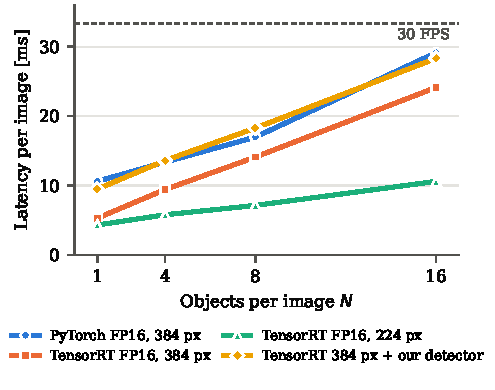
\includegraphics[width=\linewidth]{figures/latency.pdf}
  \caption{\textbf{Latency per image vs.\ number of objects} (pose pipeline from the decoded image
  to $N$ poses; LM-O model, one A100). With TensorRT FP16 and our detector, the full method stays
  above 30 FPS up to 16 objects.}
  \label{fig:supp:latency}
\end{figure}

\todo{Jetson Orin latency, if a device becomes available.}

% ---------------------------------------------------------------------------------------------
\section{Depth bias on real YCB-V images}
\label{sec:supp:depth}
\Cref{fig:supp:depth} shows the relative depth error of every test instance. On LM-O, the errors
are centred on zero (median $-0.1$\,\%, 48\,\% of the instances too far, median absolute error
1.9\,\%). On YCB-V, the whole distribution is shifted: median $+2.4$\,\%, 89\,\% of the instances
estimated too far, median absolute error 2.4\,\%. The ground-truth poses are consistent with the
depth images, so the shift means that the real YCB-V objects appear smaller in the RGB images than
their PBR renders at the same distance. A network trained on PBR images only cannot correct this
shift, which the real YCB-V training images would expose. The two weakest YCB-V objects, the wood
block (0.39 AR) and the scissors (0.41), are among the most affected (Figure~3 of the main paper
shows one example of each).

\begin{figure}[h]
  \centering
  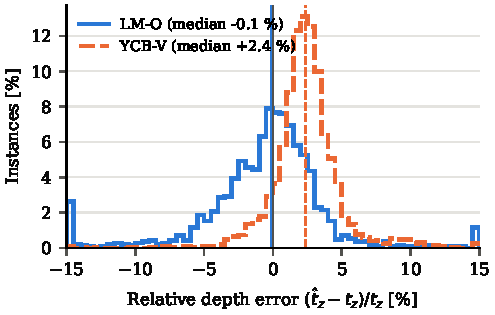
\includegraphics[width=\linewidth]{figures/depth_bias.pdf}
  \caption{\textbf{Relative depth error} $(\hat t_z - t_z) / t_z$ of all test instances with the
  default detections (LM-O: 1,445, YCB-V: 4,123), clipped at $\pm 15$\,\%; vertical lines: medians.}
  \label{fig:supp:depth}
\end{figure}

% ---------------------------------------------------------------------------------------------
\section{Per-object results}
\label{sec:supp:perobject}
Official BOP19 AR per object, computed from the per-object recalls of the BOP toolkit (the
recomputed overall AR equals the official one). ``all instances'' is the official AR; ``mean over
objects'' weighs every object equally.

\begin{table}[h]
  \centering
  \footnotesize
  \begin{tabular}{lcccc}
    \toprule
    Object & AR & VSD & MSSD & MSPD \\
    \midrule
1 ape & 0.696 & 0.486 & 0.684 & 0.917 \\
5 can & 0.826 & 0.685 & 0.850 & 0.944 \\
6 cat & 0.632 & 0.434 & 0.568 & 0.895 \\
8 driller & 0.814 & 0.675 & 0.862 & 0.906 \\
9 duck & 0.644 & 0.499 & 0.541 & 0.892 \\
10 eggbox & 0.357 & 0.169 & 0.263 & 0.639 \\
11 glue & 0.648 & 0.459 & 0.624 & 0.861 \\
12 holepuncher & 0.690 & 0.475 & 0.682 & 0.912 \\
\midrule
all instances & 0.668 & 0.491 & 0.641 & 0.873 \\
mean over objects & 0.663 &  &  &  \\
    \bottomrule
  \end{tabular}
  \caption{LM-O, final model, default detections.}
  \label{tab:perobj_lmo}
\end{table}

\begin{table}[h]
  \centering
  \footnotesize
  \begin{tabular}{lcccc}
    \toprule
    Object & AR & VSD & MSSD & MSPD \\
    \midrule
1 ape & 0.715 & 0.511 & 0.706 & 0.929 \\
5 can & 0.836 & 0.705 & 0.862 & 0.940 \\
6 cat & 0.644 & 0.448 & 0.571 & 0.912 \\
8 driller & 0.827 & 0.696 & 0.871 & 0.914 \\
9 duck & 0.670 & 0.532 & 0.579 & 0.900 \\
10 eggbox & 0.432 & 0.230 & 0.321 & 0.744 \\
11 glue & 0.669 & 0.480 & 0.654 & 0.874 \\
12 holepuncher & 0.681 & 0.466 & 0.662 & 0.913 \\
\midrule
all instances & 0.689 & 0.514 & 0.660 & 0.892 \\
mean over objects & 0.684 &  &  &  \\
    \bottomrule
  \end{tabular}
  \caption{LM-O, final model, ground-truth boxes (oracle).}
  \label{tab:perobj_lmo_gt}
\end{table}

\begin{table}[h]
  \centering
  \footnotesize
  \begin{tabular}{lcccc}
    \toprule
    Object & AR & VSD & MSSD & MSPD \\
    \midrule
1 master chef can & 0.652 & 0.553 & 0.592 & 0.810 \\
2 cracker box & 0.811 & 0.768 & 0.822 & 0.843 \\
3 sugar box & 0.767 & 0.672 & 0.759 & 0.870 \\
4 tomato soup can & 0.662 & 0.533 & 0.608 & 0.845 \\
5 mustard bottle & 0.771 & 0.666 & 0.766 & 0.881 \\
6 tuna fish can & 0.741 & 0.617 & 0.691 & 0.914 \\
7 pudding box & 0.811 & 0.654 & 0.831 & 0.947 \\
8 gelatin box & 0.716 & 0.593 & 0.620 & 0.935 \\
9 potted meat can & 0.520 & 0.444 & 0.462 & 0.655 \\
10 banana & 0.835 & 0.757 & 0.890 & 0.859 \\
11 pitcher base & 0.797 & 0.789 & 0.836 & 0.764 \\
12 bleach cleanser & 0.776 & 0.731 & 0.796 & 0.803 \\
13 bowl & 0.741 & 0.646 & 0.791 & 0.787 \\
14 mug & 0.648 & 0.487 & 0.575 & 0.883 \\
15 power drill & 0.772 & 0.675 & 0.789 & 0.852 \\
16 wood block & 0.386 & 0.232 & 0.233 & 0.692 \\
17 scissors & 0.411 & 0.153 & 0.261 & 0.817 \\
18 large marker & 0.571 & 0.322 & 0.479 & 0.911 \\
19 large clamp & 0.643 & 0.438 & 0.657 & 0.835 \\
20 extra large clamp & 0.689 & 0.532 & 0.771 & 0.764 \\
21 foam brick & 0.536 & 0.316 & 0.376 & 0.917 \\
\midrule
all instances & 0.702 & 0.591 & 0.681 & 0.834 \\
mean over objects & 0.679 &  &  &  \\
    \bottomrule
  \end{tabular}
  \caption{YCB-V, final model, default detections.}
  \label{tab:perobj_ycbv}
\end{table}


% ---------------------------------------------------------------------------------------------
\section{Reproducibility}
\label{sec:supp:repro}
All experiments use the public BOP data (PBR training images, test images, BOP19 targets, default
detections of the 2023 challenge) and the official BOP toolkit. Each configuration is trained with
two sampler seeds, and every number in the paper comes from the weights of the last epoch.
\Cref{tab:supp:repro} lists the scripts that produce the results. \todo{Repository URL and
released weights.}

\begin{table}[h]
  \centering
  \footnotesize
  \begin{tabular}{ll}
    \toprule
    Result & Script (repository) \\
    \midrule
    LM-O / YCB-V final models & \texttt{scripts/m4\_multi.sh}, \texttt{scripts/m8\_ycbv.sh} \\
    T-LESS & \texttt{scripts/m10\_tless.sh} \\
    Ablations (one change each) & \texttt{scripts/m10\_ablations.sh} \\
    Pose estimation, BOP CSV & \texttt{src/bop\_evaluate.py} \\
    Official BOP19 AR & \texttt{scripts/bop\_eval.sh} (BOP toolkit) \\
    ONNX / TensorRT, latency & \texttt{optimization/bop\_\{export,trt,latency\}.py} \\
    Detector (train, TensorRT) & \texttt{scripts/m9\_det.sh}, \texttt{optimization/bop\_det\_trt.py} \\
    Figures & \texttt{vis/paper\_*.py} \\
    \bottomrule
  \end{tabular}
  \caption{\textbf{Scripts} producing the results of the paper.}
  \label{tab:supp:repro}
\end{table}

\paragraph{Backward compatibility.}
The multi-object code keeps the single-object SPEED pipeline of FastPose-ViT unchanged: the
published SPEED model reproduces its test score (0.0093) exactly.

% ---------------------------------------------------------------------------------------------
\section{RGB-D variant}
\label{sec:supp:rgbd}
When the test depth image is available, we correct the distance of each RGB estimate and keep its
rotation. The model points of the object (the BOP evaluation models, 2,000--18,000 points) are
projected with the current pose $(\R, \T)$; a coarse z-buffer on cells of $4 \times 4$ pixels keeps
the points of the visible surface (within 5\,\% of the diameter of the front of their cell); on the
visible points whose measured depth $d_m$ is valid and agrees with their predicted depth $d_p$,
$|d_m - d_p| < \beta\, t_z$ (which drops occluders in front of the object and background behind
it), we take $\delta = \mathrm{median}(d_m - d_p)$ and move the object along its viewing ray,
$\T \leftarrow \T\, (t_z + \delta) / t_z$, which keeps the projection of its centre. Three
iterations with $\beta = 0.2, 0.1, 0.05$; estimates with fewer than 50 agreeing points keep their
RGB pose (about 1\,\% on LM-O, $<$\,0.1\,\% on YCB-V). All estimates of an image are processed
together in a few batched PyTorch operations on the GPU: 3.2\,ms (LM-O) and 3.1--4.0\,ms (YCB-V)
median per image on one A100, from the decoded depth image. A reference implementation that renders
the depth with the BOP toolkit (one render per estimate and iteration) gives the same AR (LM-O 0.750
vs.\ 0.749) at about 85\,ms per image. The median shift is $\approx 0$ on LM-O (median absolute
shift 18\,mm) and $-21$\,mm on YCB-V, the depth bias of \cref{sec:supp:depth}.

\begin{table}[h]
  \centering
  \setlength{\tabcolsep}{3pt}
  \footnotesize
  \begin{tabular}{llccccc}
    \toprule
    Dataset & RGB input & RGB AR & RGB-D AR & VSD & MSSD & MSPD \\
    \midrule
    LM-O & seed a & 0.669 & 0.749 & 0.592 & 0.786 & 0.870 \\
    LM-O & seed b & 0.664 & 0.752 & 0.596 & 0.786 & 0.874 \\
    LM-O & own LW-DETR, TensorRT & 0.654 & 0.738 & 0.590 & 0.777 & 0.847 \\
    YCB-V & seed a & 0.694 & 0.849 & 0.795 & 0.904 & 0.847 \\
    YCB-V & seed b & 0.702 & 0.851 & 0.797 & 0.908 & 0.849 \\
    T-LESS & seeds a / b & \pending{} & \pending{} & & & \\
    \bottomrule
  \end{tabular}
  \caption{\textbf{RGB-D variant} of every RGB result (default detections unless stated). With our
  detector and TensorRT, the whole RGB-D pipeline takes 24\,ms per image.}
  \label{tab:supp:rgbd}
\end{table}

{\small
\IfFileExists{ieeenat_fullname.bst}{\bibliographystyle{ieeenat_fullname}}{%
  \IfFileExists{ieee_fullname.bst}{\bibliographystyle{ieee_fullname}}{\bibliographystyle{ieeetr}}}
\bibliography{references}
}

\end{document}
